\documentclass[oneside]{article}
\author{Nathanael Chwojko-Srawley}
\title{Why Invariant is Important}


%  ╔══════════════════════════════════════════════════════════╗
%  ║                         packages                         ║
%  ╚══════════════════════════════════════════════════════════╝

\usepackage{inputenc}         % Used to compile any UTF-8 Character (and supports Unicode)
\usepackage{extarrows}         % Used to compile any UTF-8 Character (and supports Unicode)
\usepackage{stackengine}
\usepackage{scalerel}
\usepackage{amsmath, amssymb} % Used to write better mathematical expressions (ex. \mathbb{R})
\usepackage{stackrel}         % for left-right arrows, staking symbol above and bellow
\usepackage{mathrsfs}
\usepackage{euscript}
\usepackage[font=itshape]{quoting}
\usepackage{mathtools}
  \usepackage{enumitem}
\usepackage{amsthm}           % Used to create theorem enviroments.
\usepackage{graphicx}         % Let's you use images in LaTeX; ex the \includegraphics command.
\usepackage{hhline}
%\usepackage{luatexja}
%\usepackage{fontspec}
\usepackage{dsfont}
\usepackage{wasysym}          % emoji's!
\usepackage{float}            % package with ``H'' for figures and tables, ex. Images, tables, etc
%\usepackage{subcaption}      % More options with sub-captions.
\usepackage{setspace}         % More flexibility on spacing in document.
\usepackage{hyperref}         % let's me put hyperlinks
%\usepackage{tikz}             % for commutative diagrams https://tex.stackexchange.com/questions/419221/how-to-do-the-pushout-with-universal-property
\usepackage{tikz-cd}          % for commutative diagrams https://tex.stackexchange.com/questions/419221/how-to-do-the-pushout-with-universal-property
%\usepackage{quiver}           % for better commutative diagrams
\usepackage{bookmark}         % creating heading shortcut bar on the left as in word
\usepackage{longtable}        % create tables that extend past one page
%\usepackage{siunitx}         % required for alignment
%\usepackage{multirow}        % for multiple rows
\usepackage{microtype}        % makes nice text. Fixes some under-/over- filled box problems.
%\usepackage{fancyvrb}        % Let's you write code (different style than listings).
\usepackage[most]{tcolorbox} 	      % Makes nice boxes for thms, cor, prop, or anything else.
%\usepackage{enumitem}        % More flexibility on enumeration (don't know much).
\usepackage{xcolor}           % Colour text.
\usepackage{wrapfig}          % To wrap text around figure
\usepackage{listings}         % Create nice colour code blocks (customized in preamble)
\usepackage{thmtools}         % Customize theorem environment (in preamble).
%\usepackage{marvosym}        % Provide ``basic'' symbols (hazard, religious, smiley face etc.)
\usepackage{array}            % \begin{table}{>{\em}c c} -> 1st column italic (bfseries for bold)
%\usepackage[english]{babel}  % If I want to blindtext in english.
\usepackage{blindtext}
\usepackage[a4paper, total={6in, 8.5in}]{geometry}
%\usepackage[symbol]{footmisc} % For daggers and asterisk for footnotes. 1: *, 2: dagger, etc.
\usepackage{fancyhdr}
\usepackage{titlesec}
%\usepackage{pst-plot}          %To make nice plots: https://tex.stackexchange.com/questions/47594/how-can-i-make-a-graph-of-a-function#47596
% \usepackage[answerdelayed]{exercise}
\usepackage{etoolbox}          % for Dynkin diagrams
\usepackage{dynkin-diagrams}   % for Dynkin diagrams

% \usepackage{CJKutf8} % for some chinese

% to import figures via: https://github.com/gillescastel/inkscape-figures
\usepackage{import}
\usepackage{pdfpages}
\usepackage{transparent}

% This command is the ONLY command imported via the packages snippet, think of it as a tiny package written out
\newcommand{\incfig}[2][1]{%
    \def\svgwidth{#1\columnwidth}
    \import{./figures/}{#2.pdf_tex}
}

\pdfsuppresswarningpagegroup=1

\newcommand\scalemath[2]{\scalebox{#1}{\mbox{\ensuremath{\displaystyle #2}}}}
\newcommand{\Equiv}[1]{\equiv_{\scalemath{0.6}{#1}}}
\newcommand{\Plus}[1]{+_{\scalemath{0.6}{#1}}\,}
\newcommand{\Minus}[1]{-_{\scalemath{0.6}{#1}}\,}
\newcommand{\Cdot}[1]{\cdot{\scalemath{0.6}{#1}}\,}
%  ╔══════════════════════════════════════════════════════════╗
%  ║                     Custom Commands                      ║
%  ╚══════════════════════════════════════════════════════════╝

% mathbb
\newcommand{\A}{\mathbb{A}}
\newcommand{\C}{\mathbb{C}}
\newcommand{\F}{\mathbb{F}}
\newcommand{\N}{\mathbb{N}}
\newcommand{\Q}{\mathbb{Q}}
\newcommand{\R}{\mathbb{R}}
\newcommand{\V}{\mathbb{V}}
\newcommand{\Z}{\mathbb{Z}}
\renewcommand{\H}{\mathbb{H}}

% mathcal
\newcommand{\co}{\mathfrak{o}} %mathcal{o} looks like wreath product, so I changed it to mathfrak
\newcommand{\CA}{\mathcal{A}}
\newcommand{\CB}{\mathcal{B}}
\newcommand{\CC}{\mathcal{C}}
\newcommand{\CD}{\mathcal{D}}
\newcommand{\CF}{\mathcal{F}}
\newcommand{\CG}{\mathcal{G}}
\newcommand{\CH}{\mathcal{H}}
\newcommand{\CI}{\mathcal{I}}
\newcommand{\CL}{\mathcal{L}}
\newcommand{\CN}{\mathcal{N}}
\newcommand{\CO}{\mathcal{O}}
\newcommand{\CP}{\mathbb{C}\mathrm{P}}
\newcommand{\CQ}{\mathcal{Q}}
\newcommand{\CR}{\mathcal{R}}
\newcommand{\CK}{\mathcal{K}}
\newcommand{\CS}{\mathcal{S}}
\newcommand{\CT}{\mathcal{T}}
\newcommand{\CV}{\mathcal{V}}
\newcommand{\CZ}{\mathcal{Z}}

%mathscr
\newcommand{\ff}{\mathscr{F}}

%Euscript
\newcommand{\EF}{\EuScript{F}}
\newcommand{\EL}{\EuScript{L}}
\newcommand{\EO}{\EuScript{O}}
\newcommand{\EC}{\EuScript{C}}

%mathfrak (lowercase)
\newcommand{\fa}{\mathfrak{a}}
\newcommand{\fb}{\mathfrak{b}}
\newcommand{\fc}{\mathfrak{c}}
\newcommand{\fd}{\mathfrak{d}}
\newcommand{\fm}{\mathfrak{m}}
\newcommand{\fn}{\mathfrak{n}}
\newcommand{\fo}{\mathfrak{o}}
\newcommand{\fp}{\mathfrak{p}}
\newcommand{\fq}{\mathfrak{q}}

%mathfrak (upper case)
\newcommand{\FA}{\mathfrak{A}}
\newcommand{\FB}{\mathfrak{B}}
\newcommand{\FP}{\mathfrak{P}}
\newcommand{\FC}{\mathfrak{C}}
\newcommand{\FD}{\mathfrak{D}}
\newcommand{\FM}{\mathfrak{M}}
\newcommand{\FN}{\mathfrak{N}}
\newcommand{\FO}{\mathfrak{O}}

% operatorname
\newcommand{\ev}{\operatorname{ev}}
\newcommand{\tr}{\operatorname{tr}}
\newcommand{\nm}{\operatorname{Nm}}
\newcommand{\op}{\operatorname{op}}
\newcommand{\ad}{\operatorname{ad}}
\newcommand{\im}{\operatorname{im}}
\newcommand{\id}{\operatorname{id}}
\newcommand{\ch}{\operatorname{ch}}
\newcommand{\ab}{\operatorname{ab}}
\newcommand{\SL}{\operatorname{SL}}
\newcommand{\GL}{\operatorname{GL}}
\renewcommand{\Re}{\operatorname{Re}}
\renewcommand{\Im}{\operatorname{Im}}
\newcommand{\rad}{\operatorname{rad}}
\newcommand{\vol}{\operatorname{vol}}
\newcommand{\Gal}{\operatorname{Gal}}
\newcommand{\Rep}{\operatorname{Rep}}
\newcommand{\Aut}{\operatorname{Aut}}
\newcommand{\Sym}{\operatorname{Sym}}
\newcommand{\Mod}{\operatorname{Mod}}
\newcommand{\Grp}{\operatorname{Grp}}
\newcommand{\Hom}{\operatorname{Hom}}
\newcommand{\Emb}{\operatorname{Emb}}
\newcommand{\Ext}{\operatorname{Ext}}
\newcommand{\End}{\operatorname{End}}
\newcommand{\Inn}{\operatorname{Inn}}
\newcommand{\Ind}{\operatorname{Ind}}
\newcommand{\Out}{\operatorname{Out}}
\newcommand{\Jac}{\operatorname{Jac}}
\newcommand{\Nil}{\operatorname{Nil}}
\newcommand{\Tor}{\operatorname{Tor}}
\newcommand{\Ann}{\operatorname{Ann}}
\newcommand{\Syl}{\operatorname{Syl}}
\newcommand{\Res}{\operatorname{Res}}
\newcommand{\lcm}{\operatorname{lcm}}
\newcommand{\conj}{\operatorname{conj}}
\newcommand{\disc}{\operatorname{disc}}
\newcommand{\stab}{\operatorname{stab}}
\newcommand{\kdim}{\operatorname{kdim}}
\newcommand{\coker}{\operatorname{coker}}
\newcommand{\Obj}{\operatorname{Obj}}
\newcommand{\Mor}[1]{\operatorname{Mor}(\textbf{#1})}
\newcommand{\Frac}{\operatorname{Frac}}
\newcommand{\Frob}{\operatorname{Frob}}
\newcommand{\Spec}{\operatorname{Spec}}
\newcommand{\mSpec}{\operatorname{mSpec}}
\newcommand{\Char}{\operatorname{char}}
\newcommand{\fHom}[1]{\operatorname{Hom}(#1, \_\_)}
\newcommand{\cofHom}[1]{\operatorname{Hom}(\_\_, #1)}
\newcommand{\trdeg}{\operatorname{trdeg}}
\newcommand{\Span}{\operatorname{span}}

%shorthands
\renewcommand{\bf}[1]{\textbf{#1}}
\newcommand{\qn}{\quad\newline}
\newcommand{\oln}{\overline}
\renewcommand{\phi}{\varphi}
\newcommand{\placeholder}{\_\_\_\_\_}
\newcommand{\set}[2]{\left\{#1 \ \middle|\ #2\right\}}

% connectors
\renewcommand{\mid}{\big|}
\newcommand{\sse}{\subseteq}
\newcommand{\subg}{\leqslant}
\newcommand{\supg}{\geqslant}
\newcommand{\ssne}{\subsetneq}
\newcommand{\isosubg}{\lesssim}
\newcommand{\nsse}{\not\subseteq}
\newcommand{\nsubg}{\trianglelefteq}
\newcommand{\nsupg}{\trianglerighteq}
\newcommand{\csubg}{\blacktriangleleft}
%\newcommand{\subgne}{\lneqslant}

% limits
\newcommand{\Lim}{\varprojlim}
\newcommand{\colim}{\varinjlim}
\newcommand{\coLim}{\varinjlim}
\newcommand{\Dlim}{\lim\limits_{\longrightarrow}}
\newcommand{\coDlim}{\lim\limits_{\longleftarrow}}


%for saturated ideals in the localization section (I don't like these, I think I'll delete)
\newcommand{\LIm}{{}^{\iota} }
\newcommand{\LPre}{{}^{\pi} }

% Arrows
\newcommand{\rw}{\rightarrow}
\newcommand{\Rw}{\Rightarrow}
\newcommand{\lw}{\leftarrow}
\newcommand{\Lw}{\Leftarrow}
\newcommand{\lrw}{\leftrightarrow}
\newcommand{\LRw}{\Leftrightarrow}
\newcommand{\rrw}{\rightrightarrows}
\newcommand{\acton}{\curvearrowright}
\newcommand{\actson}{\curvearrowright}
\newcommand\mapsfrom{\mathrel{\reflectbox{\ensuremath{\mapsto}}}}

% dcups
\newcommand{\dcup}{\sqcup}
\newcommand{\Dcup}{\bigsqcup}

%a nice large circle
\newcommand{\tikzcircle}[2][red,fill=black]{\tikz[baseline=-0.5ex]\draw[#1,radius=#2] (0,0) circle ;}%
\makeatletter
\newcommand*\bigcdot{\mathpalette\bigcdot@{.5}}
\newcommand*\bigcdot@[2]{\mathbin{\vcenter{\hbox{\scalebox{#2}{$\m@th#1\bullet$}}}}}
\makeatother

%somehow not a default command
\def\rddots{\mathstrut^{.^{.^{.}}}}

%% new delimiter
\DeclarePairedDelimiter{\ceil}{\lceil}{\rceil}


%  ╔══════════════════════════════════════════════════════════╗
%  ║                          proofs                          ║
%  ╚══════════════════════════════════════════════════════════╝
\usepackage{tikz-cd}          % for commutative diagrams https://tex.stackexchange.com/questions/419221/how-to-do-the-pushout-with-universal-property
\def\exampletext{Exercise} % If English
\colorlet{colexam}{red!55!black} % Global example color


\newtcbtheorem{exercise}{Exercise}{% \newtcolorbox[use counter=testexample]{testexamplebox}{%
% Example Frame Start
empty,% Empty previously set parameters
title={\exampletext \thetcbcounter #1},% use \thetcbcounter to access the testexample counter text
% Attaching a box requires an overlay
attach boxed title to top left,
   % Ensures proper line breaking in longer titles
   minipage boxed title,
% (boxed title style requires an overlay)
boxed title style={empty,size=minimal,toprule=0pt,top=4pt,left=3mm,overlay={}},
coltitle=colexam,fonttitle=\bfseries,
before=\par\medskip\noindent,parbox=false,boxsep=0pt,left=3mm,right=0mm,top=2pt,breakable,pad at break=0mm,
   before upper=\csname @totalleftmargin\endcsname0pt, % Use instead of parbox=true. This ensures parskip is inherited by box.
% Handles box when it exists on one page only
overlay unbroken={\draw[colexam,line width=.5pt] ([xshift=-0pt]title.north west) -- ([xshift=-0pt]frame.south west); },
% Handles multipage box: first page
overlay first={\draw[colexam,line width=.5pt] ([xshift=-0pt]title.north west) -- ([xshift=-0pt]frame.south west); },
% Handles multipage box: middle page
overlay middle={\draw[colexam,line width=.5pt] ([xshift=-0pt]frame.north west) -- ([xshift=-0pt]frame.south west); },
% Handles multipage box: last page
overlay last={\draw[colexam,line width=.5pt] ([xshift=-0pt]frame.north west) -- ([xshift=-0pt]frame.south west); }%
}{ex}


\def\prooftext{Proof} % If English
\NewDocumentEnvironment{Proof}{ O{} }
{
  \colorlet{colexam}{black!55!black} % Global example color
  \newtcolorbox[number within=section]{testproofbox}{% \newtcolorbox[use counter=testexample]{testexamplebox}{%
    % Example Frame Start
    empty,% Empty previously set parameters
    title={\emph{\prooftext} \thetcbcounter: #1},% use \thetcbcounter to access the testexample counter text
    % Attaching a box requires an overlay
    attach boxed title to top left,
       % Ensures proper line breaking in longer titles
       minipage boxed title,
    % (boxed title style requires an overlay)
    boxed title style={empty,size=minimal,toprule=0pt,top=4pt,left=3mm,overlay={}},
    coltitle=colexam,fonttitle=\bfseries,
    before=\par\medskip\noindent,parbox=false,boxsep=0pt,left=3mm,right=0mm,top=2pt,breakable,pad at break=0mm,
       before upper=\csname @totalleftmargin\endcsname0pt, % Use instead of parbox=true. This ensures parskip is inherited by box.
    % Handles box when it exists on one page only
    overlay unbroken={\draw[colexam,line width=.5pt] ([xshift=-0pt]title.north west) -- ([xshift=-0pt]frame.south west); },
    % Handles multipage box: first page
    overlay first={\draw[colexam,line width=.5pt] ([xshift=-0pt]title.north west) -- ([xshift=-0pt]frame.south west); },
    % Handles multipage box: middle page
    overlay middle={\draw[colexam,line width=.5pt] ([xshift=-0pt]frame.north west) -- ([xshift=-0pt]frame.south west); },
    % Handles multipage box: last page
    overlay last={\draw[colexam,line width=.5pt] ([xshift=-0pt]frame.north west) -- ([xshift=-0pt]frame.south west); },%
    }
  \begin{testproofbox}
}
{\end{testproofbox}\endlist}

\newtcbtheorem[number within=section]{titledBox}{}{%
  enhanced,
  sharp corners,
  colback=white,
  colframe=black,
  borderline={0.2pt}{0pt}{black},
  left=2mm,
  right=2mm,
  top=2mm,
  bottom=2mm,
  title style={opacity=1},
  attach title to upper,
  before upper={\textbf{\tcbtitletext}\quad},
  coltitle=black,
  fonttitle=\bfseries,
  separator sign={\quad}
}{box}
\setlength{\parindent}{0pt} % don't like indentation infront of paragraphs
\setlength{\parskip}{1ex}   %so that there is still space between paragarphs

% \usepackage[backend=biber,citestyle=alphabetic,bibstyle=authortitle]{biblatex}
\usepackage{biblatex}

\addbibresource{bibliography.bib}

\makeatletter
\def\blfootnote{\gdef\@thefnmark{}\@footnotetext}
\makeatother



\begin{document}

\begin{center}
  \Huge{Clock Arithmetic and the Mysteries of Prime Numbers}
\end{center}

\begin{titledBox*}{Foreword}
  \qn
  This article is written for my patient friends to whom I give math riddles that require knowledge of modular
  arithmetic, or as I often call it \emph{clock arithmetic}. This article serves as an easy reference for the
  necessary concepts and requires no mathematical background. For this entire article, we will only care about
  which hour the hour-hand is on; no AM or PM, and no adding half an hour (or anything that isn't an increment
  of 60 minutes).

  \qn
  Note that any exercise can be skipped; they are just there for fun!
\end{titledBox*}

\section{Clock Arithmetic: Addition and Multiplication}


We all have (at least) two ideas of addition in our heads. The first one is the usual notion of adding
quantities\footnote{A mathematician would say \emph{discrete quantities} to distinguish between
  \emph{continuous} quantities, which would describe something like water where the amount we add is on a
``continuous'' spectrum of possible amounts rather than ``discrete'' indivisible chunks of amounts}: If I have
$4$ bottles and add $10$ bottles, I have $14$ bottles. In other words
\[
  4+10 = 14
\]
The other notion of addition we often use comes from when we are calculating what time it is. Consider a
$12$-hour clock. If it is $4$ o-clock, in $5$ hours it will be $9$ o-clock. If instead we add $10$ hours, it
will be $2$ o-clock. In other words, we just comfortably did
\[
  4+10 = 2
\]
in our heads. This is certainly different from before, but it still makes sense! Using the same symbol ``$+$''
may cause confusion, so to distinguish the two types of addition, we shall write $+_{12}$ for ``12 hour
clock'' addition, and keep $+$ as before. Thus, we can write:
\[
  4+10 = 14 \qquad \text{and} \qquad 4+_{12}10 = 2
\]
Let us call the addition using $+$ \emph{natural arithmetic} and the addition using $+_{12}$
\emph{clock arithmetic}. As good mathematicians, we should see what similarities and differences these
different ideas of additions have.

The first thing we should try to do is add a bunch of hours to each other and see what we get. Let us start by
just picking two random numbers and playing around with them. If it is $2$ o-clock, then if I add $5$ it will
be $7$ o-clock. But if I add $17$, it will \emph{still} be $7$ o-clock. More generally, adding any multiple of
$12$ will not change the result of my addition:
\[
  2\Plus{12} 5 = 7,\quad 2\Plus{12}17 = 7, \quad 2\Plus{12}29=7,\quad 2\Plus{12}41 = 7\cdots
\]
So adding $5,(5+1\cdot 12), (5+2\cdot 12), ...$ to $2$ gives the same result. Similarly, if I have any number $a$ between
$1$ and $12$, if I add $b$, or I add $(b + k\cdot 12)$ for some $k = 1,2,...$ I get the same result.

We would like to remember that adding a number $n$ or adding a number
$n+k\cdot 12$ gives the same result. Mathematicians usually use the symbol $\Equiv{12}$ between two such
numbers:
\[
  5\Equiv{12}17\Equiv{12}29\Equiv{12}\cdots
\]
where we usually say that $5$ is \emph{equivalent} to $17$, which is equivalent to $29$, and so forth. Said
differently, two numbers $a,b$ are equivalent if they give you the same time on the clock-face after adding:
\[
  n\Plus{12}a = m \qquad \text{and} \qquad n\Plus{12}b= m
\]
Therefore, in clock arithmetic we only need to work with the following numbers:
\[
  1,2,3,4,5,6,7,8,9,10,11,12
\]
All these numbers are \emph{not} equivalent to each other (ex. $3\not\Equiv{12}5$). Adding any two of these
numbers using $+_{12}$ will give another number in the above list:
\[
  1\Plus{12}1 = 2\qquad 11\Plus{12}7 = 6 \qquad 9\Plus{12}12 = 9
\]
The last of these three examples is somehow different than the others; it is the only equation where one of
the numbers on the left hand side of the addition $+_{12}$ also appears on the right hand side of the
equality; namely $9$ appears on both sides. In fact, if we try adding any other number to $9$, we see that only adding $12$ returns $9$:
\[\begin{array}{|lcl|lcl|lcl|}
  \hline
9\Plus{12}1 &=& 10 & 9\Plus{12}5 &=& 2 & 9\Plus{12}9 &=& 6 \\
9\Plus{12}2 &=& 11 & 9\Plus{12}6 &=& 3 & 9\Plus{12}10 &=& 7 \\
9\Plus{12}3 &=& 12 & 9\Plus{12}7 &=& 4 & 9\Plus{12}11 &=& 8 \\
9\Plus{12}4 &=& 1 & 9\Plus{12}8 &=& 5 & 9\Plus{12}12 &=& 9\\
\hline
\end{array}\]

The natural next question to ask is if this works for any number, not just $9$. Try doing this for any $n$
between $1$ and $12$ (including $12$), and you'll see that adding $12$ to any number gives back the same
number, and $12$ is the \emph{only} number that does this!
\[
  n \Plus{12}12 = n
\]
Notice that in natural arithmetic, this is exactly the behaviour of $0$! Namely, for any natural number $n$:
\[
  n + 0 = n
\]
With this parallel in mind, when we are doing clock arithmetic, we should think of $12$ as being the same
as $0$. Mathematicians would even go so far as re-labeling $12$ as $0$ so that the $12$ numbers of
clock arithmetic are:
\[
  0,1,2,3,4,5,6,7,8,9,10,11
\]
Re-labeling $12$ as $0$ has another advantage when we consider \emph{multiplication} in clock arithmetic.
If we are to think of $12$ as being $0$ in clock arithmetic, we should at least check that this behavior is also respected by multiplication. Remember that in natural arithmetic,
multiplying any number $n$\footnote{For those who have contested this by asking ``what if we let $n$ be
  infinity'', there is \href{NOT_YET}{this article} addressing exactly how to think about infinity and why we
shouldn't conclude $0\cdot \infty = 0$ without putting in more care} by $0$ gives $0$:
\[
  n\cdot 0 = 0
\]
Let us first test if this is the case by doing an example. If it is $3$ o-clock and we
multiply by $12$, then we are adding $3$ o-clock to itself $12$ times, which would bring us $36$ hours
forward, which on a clock-face is $12$ o-clock. But we already saw that we should think of $12$ as being
$0$! Hence, we see that adding $3$ to itself $12$ times will give us back $0$. In fact, if we start with any
number $n$ between $0$ and $11$, adding the number to itself $12$ times will always bring us back to the $12$
o-clock position! Therefore, $12$ really \emph{does} behave like $0$ in clock arithmetic! If $\cdot_{12}$
represents multiplication in clock arithmetic, we just showed that multiplying by 12 is like multiplying by 0. For example:
\[
  3\Cdot{12}12 = 12
\]
Which in our re-labeled system (where 12 is 0) becomes:
\[
  3\Cdot{12}0 = 0
\]
\begin{exercise}{Multiplying by other numbers}{zeroDiv}
  When multiplying in natural arithmetic we get that $a\cdot b= 0$ if and only if $a = 0$ or $b= 0$. In
  clock arithmetic, it is now possible that $a\cdot_{12}b=  0$ but $a,b \ne 0$! Can you think of two
  non-zero numbers $a,b$ where $a\cdot_{12}b = 0$?
\end{exercise}


\begin{exercise}{Combining Addition and Multiplication}{distributivity}
  Show that for any natural numbers $a,b,c$
  \[
    a\cdot_{12}(b+_{12}c) = (a\cdot_{12}b) +_{12} (a\cdot_{12}c)
  \]
  \vspace{0.5em}
  \blfootnote{Mathematicians call this \emph{distributivity}}
\end{exercise}

\begin{exercise}{Subtraction}{subtraction}
  Subtraction works just the same as addition. Convince yourself that:
  \[
    1\Minus{12}2 = 11
  \]
  that is, if it is $1$ o-clock, two hours ago it was $11$ o-clock. Convince yourself that:
  \[
    a\Minus{12}12 = a
  \]
\end{exercise}

\newpage
\section{From Clock Arithmetic to Modular Arithmetic}

So we just showed how we can think of clock arithmetic which has $12$ numbers.
A mathematician would then naturally ask the following question:
\begin{center}
  What if we replace $12$ with any other natural number\footnote{A natural number is of the form $1,2,3,...,
  n,...$. We in fact \emph{can} replace it with non-natural numbers, but it took some time in history to
  understand what this means; this would be introduced in a course in \emph{abstract algebra}
  (see\cite{NateAlgebra} if you want my exposition on abstract algebra)}?
\end{center}
Let us do exactly this and see what we get! First off, instead of writing $+_{12}$, we shall now write
$+_{n}$. Let us call the arithmetic for all $+_{n}$ \emph{modular arithmetic}. With this vocabulary,
clock arithmetic is a special case of modular arithmetic. To distinguish the different modular arithmetics, we
would usually say we are working \emph{modulo $n$}. Clock arithmetic would be modular arithmetic modulo
$12$. When working modulo $n$, we can imagine a clock face with $n$ positions. For example, if $n =5$, then we
can think of having a clock with $5$ hours:
\[
  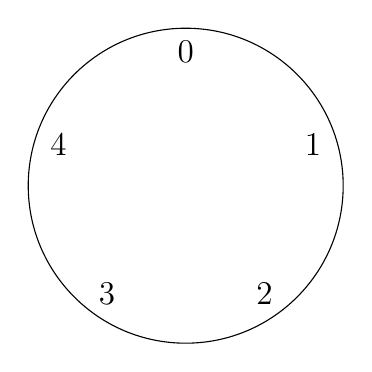
\begin{tikzpicture}
    % Draw the main circle
    \draw (0,0) circle (2cm);

    % Place the numbered points at equal angles
    % Starting from 90° (top) and moving clockwise
    % Each point is 72° apart (360° / 5 = 72°)
    \foreach \x [count=\xi from 0] in {90,18,-54,-126,-198} {
        \node[font=\large] at ({1.7*cos(\x)},{1.7*sin(\x)}) {\xi};
    }
\end{tikzpicture}
\]
On this clock, $3+_{5}3 = 1$ and $2\cdot_{5}4 = 3$. When working modulo $n$, we will always have $n$ numbers:
\[
  0,1,2,..., n-1
\]
Just like for clock arithmetic, we have that we can treat $n$ like $0$.

\begin{exercise}{Zero in Modular Arithmetic}{0InModArithmetics}
  Let $a,n$ be any natural numbers. For a moment, let us not label $n$ as $0$. Convince yourself that:
  \[
    a\cdot_{n}n = n
  \]
  This shows that in modular arithmetic mod $n$, we can \emph{always} treat $n$ as $0$, and hence why we
  will always write $0$ instead of $n$.
\end{exercise}


\begin{exercise}{Special Property when Modulo Prime}{propModPrime}
  Remember in exercise~\ref{ex:zeroDiv} that in modulo $12$, we can find two natural numbers $a,b$ where
  $a\cdot_{12} b= 0$, but $a,b\ne 0$.

  Convince yourself that if $n = p$ is a prime number (ex. $p = 2,3,5,7,11,...$) then
  \[
    a\cdot_p b = 0 \qquad \text{if and only if} \qquad a = 0\text{ or } b= 0
  \]
  This shows that primes are somehow ``special''. Mathematicians even have a different word for when $n = p$
  is a prime: modular arithmetic modulo $p$ where $p$ is a prime is called a \emph{finite field}.
\end{exercise}

\newpage
\section{Application: Equations}

So now that we defined modular arithmetic, what can we do with it? The biggest reason mathematicians care
about modular arithmetic is that it allows us to give a lot more information about equations we are trying
to solve!

For example, consider $x^2+x+1$. If I ask you to tell me whether there is an integer $n$, numbers of the for
$\pm1, \pm2, \pm3, ...$, that solves this equation (i.e. an $n$ such that $n^2+n+1 =0$), it may take you a
little while to figure out if such a number exists. A natural starting point is to just convince yourself that
no small integer can solve it. By plugging in  $\pm1, \pm2, \pm3$ we get:
\[
\begin{array}{|c|c|c|}
\hline
x & \text{Calculation} & \text{Result} \\
\hline
1 & 1^2 + 1 + 1 & 3 \\
\hline
-1 & (-1)^2 + (-1) + 1 & 1 \\
\hline
2 & 2^2 + 2 + 1 & 7 \\
\hline
-2 & (-2)^2 + (-2) + 1 & 3 \\
\hline
3 & 3^2 + 3 + 1 & 13 \\
\hline
-3 & (-3)^2 + (-3) + 1 & 7 \\
\hline
\end{array}
\]
Doing this for the first 100 integers and their negatives would give you that the equation never equals $0$,
however there is no guarantee that you will \emph{never} find a big enough number $n$ such that $n^2+n+1=0$.
Using modular arithmetic, it is in fact straightforward to show that \emph{no} solutions exist.

To show this, let's say that there \emph{does} exist an $n$ such that $n^2+n+1=0$\footnote{This is a usual
trick called \emph{proof by contradiction}}. What we will do is show that this equation will \emph{fail} when
we consider modular arithmetic modulo $2$. In modulo $2$, the number $n$ would be equivalent to:
\[
  n\Equiv{2} 0 \qquad \text{or} \qquad n\Equiv{2}1
\]
For example, if $n = -177$ (which the reader could check doesn't solve the equation, but it is just for
demonstration), then:
\[
  -177 = 1 + 2\cdot (-89) \Equiv{2} 1
\]
(look at exercise~\ref{ex:subtraction} if the subtraction doesn't sit well with you). We can keep $1$ and $0$
the same because they happen to be small enough so that we don't need to shrink them. Thus, armed with the
possible values of $n$ modulo $2$, we get one of two possible equations:
\[
  (1\Cdot{2}1) \Plus{2} 1 \Plus{2} 1 = 0 \qquad \text{or} \qquad (0\Cdot{2}0) \Plus{2}0\Plus{2} 1 = 0
\]
But hang on, if we compute the left hand side of the first equation we get
\[
  1\Plus{2}1\Plus{2}1 = 0\Plus{2}1 = 1
\]
which is \emph{not} equal to the right hand side (i.e. $1\ne 0$ and $1\not\Equiv{2}0$). The second equation is
even more obvious since $(0\Cdot{2}0) \Plus{2}0\Plus{2} 1 = 1$ which is again not equal to $0$.

So we arrived at a contradiction, because $0\ne 1$\footnote{The suspicious reader may ask why is $0\ne 1$. In
  fact, there is nothing wrong with the arithmetic system where $0 = 1$, however if we let $0 = 1$ we get that
every number equals $0$ (convince yourself), and then nothing interesting happens.}. What this tells us is
that we made a wrong assumption earlier in the proof, and indeed this started by assuming that there exists an
integer $n$ such that $n^2+n+1=0$. Thus, it is \emph{impossible} that such an
integer exists! Notice how easy this was to prove: we only had to check \emph{2} possible numbers as
compared to the infinite possibilities when trying to solve the equation with natural numbers!

This ``reduction to finitely many cases'' is one of the \textbf{key} properties of modular arithmetic that
mathematicians abuse to no end.


\section{Application: Patterns in Prime Numbers}

Consider the equation $x^2 = p$ for some prime number $p$. Then obviously no natural number solves this
equation, because no natural number can be the square-root of a prime\footnote{This is because the square-root
  of a prime number is \emph{irrational}; see~\cite{fuchsIntroductionProofsProof} for a friendly introduction
to this notion}. However, this question gets more interesting if we instead consider it in \emph{modular
arithmetic} modulo $n$.

Let us demonstrate this with an example. Consider $p = 3$. Let us see if in modulo $n$, we can find a number
$m$ such that $m\Cdot{n} m = p$ (i.e. if $p$ has a square-root modulo $n$). The following is a table where $n$
goes over the first few prime numbers:

\begin{longtable}{|c||c|c|c|c|c|c|c|c|c|c|c|}
\hline
n & $1^2$ & $2^2$ & $3^2$ & $4^2$ & $5^2$ & $6^2$ & $7^2$ & $8^2$ & $9^2$ & $10^2$\\
\hline
2 & 1 & & & & & & & & & \\
\hline
3 & 1 & 1 & & & & & & & & \\
\hline
4 & 1 & 0 & 1 & & & & & & & \\
\hline
5 & 1 & 4 & 4 & 1 & & & & & & \\
\hline
6 & 1 & 4 & *\textbf{3}* & 4 & 1 & & & & & \\
\hline
7 & 1 & 4 & 2 & 2 & 4 & 1 & & & & \\
\hline
8 & 1 & 4 & 1 & 0 & 1 & 4 & 1 & & & \\
\hline
9 & 1 & 4 & 0 & 7 & 7 & 0 & 4 & 1 & & \\
\hline
10 & 1 & 4 & 9 & 6 & 5 & 6 & 9 & 4 & 1 & \\
\hline
11 & 1 & 4 & 9 & 5 & *\textbf{3}* & *\textbf{3}* & 5 & 9 & 4 & 1 \\
\hline
\end{longtable}

Let us focus on the cases where $n = p$ is a prime number. Notice that $5\Cdot{11}5 = 3$, since $5\cdot 5 =25
= 3+2\cdot 11$. Hence, for a mysterious reason, there \emph{does} exist a square-root of $3$ in modulo $11$,
and there \emph{doesn't} appear to be a square-root of $3$ modulo the other small primes like $5$ and $7$. There in fact
exists many other prime numbers $n$ such that $3$ has a square-root modulo $n$, infinitely many of them in fact. But
why $11$? Why was the prime $3$ somehow linked to the prime $11$?

This is a rather fascinating result: primes somehow have \emph{relations} between each other! Two primes are
somehow tied to each other depending on whether we can take the square root of one modulo the other! Euler in the 19th
century had the exact same realization, and did thousands of such computations looking for patterns. It turns out
to be a rather hard problem, and it wasn't until Gauss around 50 years later that gave a definitive and
satisfactory explanation how such primes relate via square-rooting: the result is now called \emph{quadratic
reciprocity}. Unfortunately, answering this question would require a lot more than what this article covers
(all the details are in \cite{NateAlgebra}, and requires a good deal of build-up before being proven in
chapter~22.4). However, I strongly encourage the reader play around with this; after a few hours or a few
days, the reader will most likely stumble upon the same pattern that many other mathematicians who worked
on the problem (including Euler) have discovered!
\newpage
\section{Final Mystery}


The problem in the above section turned out to be one of the first cornerstones in number theory, as it
somehow connects different prime numbers to each other via equations; that is, somehow prime numbers are not
completely ``random'' but can have subtle connections that are not obvious at first glance!

This next and final problem we shall present:
\begin{center}
  Are there infinitely or finitely many primes $p$ such that
  \[
    p-3\Equiv{5}0
  \]
  where $3$ and $5$ can be replaced with any numbers $a,b$ where $\gcd(a,b) = 1$ (i.e. they have no common
  factors).
\end{center}
 This question was pondered by Dirichlet in 1837, and essentially is asking about how prime numbers are
 ``distributed'' (i.e., is there a meaningful way in which we can group prime numbers together). Just like the
 above problem, I strongly encourage the reader to think about this problem for a couple of hours and just see
 what they can come up with. The result has been proven, and a full proof requires a good deal more than what
 can be covered in an expository article like this (though for completeness, a proof can be found
 in~\cite{NateCFT}).




\newpage
\printbibliography % needs package 'biblatex'

\end{document}

